\documentclass[11pt, oneside]{book}

% URLs and hyperlinks ---------------------------------------
\usepackage{hyperref}
\hypersetup{
    colorlinks=true,
    linkcolor=blue,
    filecolor=magenta,      
    urlcolor=blue,
}
\usepackage{xurl}
%---------------------------------------------------

% titlepage -------------------------------------------------
\usepackage{pdfpages}
%------------------------------------------------------------

% tables -------------------------------------------------------
\usepackage{float}
\usepackage{multirow}
\renewcommand{\arraystretch}{1.23}
% ---------------------------------------------------------------------

% commands --------------------------------------------
\newcommand{\amz}{\lr{Amazon} }
% -----------------------------------------------------------

\usepackage{xepersian}
\settextfont{Yas}
\setdigitfont{Yas}

\begin{document}
\frontmatter
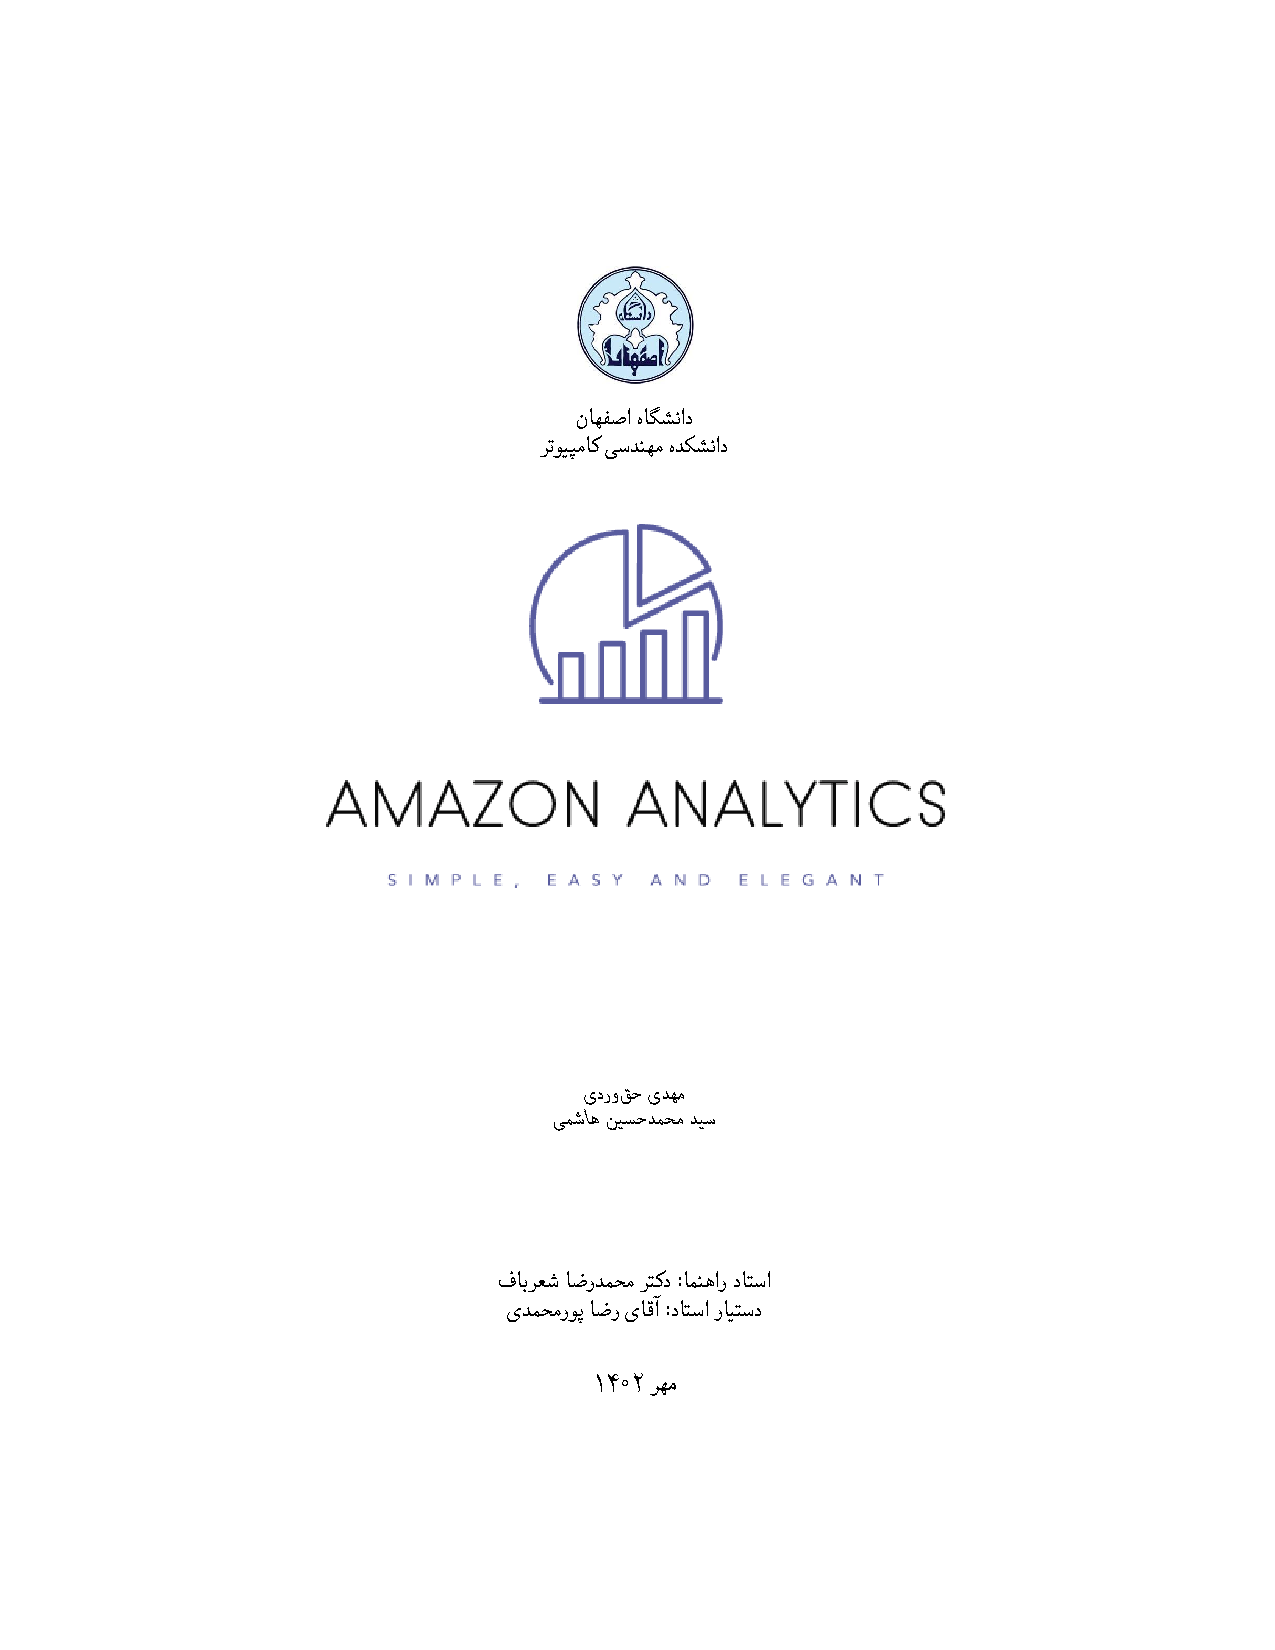
\includepdf{../titlepage/title}
\tableofcontents
\mainmatter

\chapter{ماتریس \lr{RACI}}
\begin{table}[H]
\begin{latin}
\begin{center}
\begin{tabular}{|c|c|c|c|c|}
\hline
Task/Person & Mahdi & Mohammad & Teacher & TA \\
\hline
\end{tabular}
\end{center}
\end{latin}
\end{table}

\chapter{بخش ۲، تعریف پروژه\\\lr{(Project Definition)}}
\section{دورنما \lr{(Vision)}}
\section{اهداف \lr{(Objectives)}}
\section{قلمرو \lr{(Scope)}}
\section{موارد تحویل دادنی \lr{(Deliverables)}}

\chapter{بخش ۳.۳، نقش\\\lr{(Role)}}

\chapter{بخش ۳.۴، مسئولیت‌ها\\\lr{(Responsibilities)}}

\chapter{بخش ۵، ملاحظات پروژه\\\lr{(Project Considerations)}}

\chapter{قالب \lr{Risk Assessment Matrix}}
\end{document}